\documentclass[conference]{IEEEtran}
\IEEEoverridecommandlockouts
% The preceding line is only needed to identify funding in the first footnote. If that is unneeded, please comment it out.
\usepackage{cite}
\usepackage{amsmath,amssymb,amsfonts}
\usepackage{algorithmic}
\usepackage{graphicx}
\usepackage{textcomp}
\usepackage{xcolor}
\usepackage{caption}
\usepackage{array}
\usepackage{hhline}
\usepackage{pgfplots}
\usepackage[english]{babel}
\usepackage{hyperref}
\usepackage{breakurl} % Better URL breaking for PDF-based workflows 
\hypersetup{
    colorlinks=true,
    urlcolor=blue,
    linkcolor=blue,
    filecolor=magenta,
    citecolor=blue
}
\renewcommand{\url}[1]{\uline{\textcolor{blue}{\texttt{#1}}}}
\usepackage[normalem]{ulem} % for underlining


\def\BibTeX{{\rm B\kern-.05em{\sc i\kern-.025em b}\kern-.08em
    T\kern-.1667em\lower.7ex\hbox{E}\kern-.125emX}}
\begin{document}

\title{Using Haar Feature-Based Cascade Classifiers for Face Detection on a Raspberry Pi for IoT Applications}

\author{\IEEEauthorblockN{Ethan Leyden}
\IEEEauthorblockA{\textit{Department of Computer Science} \\
\textit{Virginia Commonwealth University}\\
Richmond, VA, USA \\
leydene@vcu.edu}
\and
\IEEEauthorblockN{Alan Dorn}
\IEEEauthorblockA{\textit{Department of Computer Science} \\
\textit{Virginia Commonwealth University}\\
Richmond, VA, USA \\
dornn@vcu.edu}
\and
\IEEEauthorblockN{Cameron Clyde}
\IEEEauthorblockA{\textit{Department of Computer Science} \\
\textit{Virginia Commonwealth University}\\
Richmond, VA, USA \\
clydecp@vcu.edu}}

\maketitle

\begin{abstract}

Internet of Things (IoT) devices are frequently implemented and popular solutions for many applications, including facial detection and recognition for home security systems. \cite{OneRadzi} Raspberry Pi’s (Rpi) are small, efficient single-board computers that provide an affordable computing platform for numerous applications requiring a small physical footprint. \cite{TwoNayyar} Facial detection is the process of identifying human faces in an image. This technology has become increasingly popular as it allows for people to be efficiently tracked without any human intervention. \cite{SevenKatsanis} Haar feature-based cascade classifiers are a popular tool in the field of computer vision used for object detection. In this paper, we will explore the utility of Haar  feature-based classifiers for facial recognition on the Raspberry Pi by analyzing the performance of the algorithm, and investigating applications for face detection in this context. The researchers of this paper pose questions like “What are viable ways that Rpi’s can be implemented by non-experts in home security solutions?” and “How well does an Rpi perform as a platform for a facial recognition system?”
\end{abstract}

\begin{IEEEkeywords}
Internet Of Things; Haar feature-based cascade classifier; Facial Recognition; Raspberry Pi;
\end{IEEEkeywords}



\section{Introduction}
Face detection (the ability to recognize faces in an image) and face recognition (the ability to identify faces in an image) are well-studied computer vision tasks. The face detection problem is commonly solved using a Haar feature-based cascade classifier \cite{FiveCuimei}. The method is usually chosen for its speed and conceptual simplicity. The classifier works by moving a sliding window across an image, in a raster scan fashion. As the window slides across the image, Haar features (depicted in Figure \ref{haarfeature}) are used to perform calculations on adjacent rectangles within the window. In the training step, AdaBoost is typically used \cite{TenAras,ElevenNiranjan} to build the cascade structure in Figure \ref{cascademodel} by evaluating the best Haar features in the set. When using the model after the training step, the sliding window and set of Haar features is used again to evaluate whether the features discovered in training exist within the window, if so the computation moves down the cascade model, and the image within the face is classified as a face when most or all of the features are found in the window. The method was first used by Viola and Jones in their groundbreaking paper on rapid object detection \cite{SixViola}, demonstrating the approach to be computationally efficient. This is backed up by the 2021 literature review done by Hirzi et al \cite{NineHirzi}. Who finds that the Viola and Jones algorithm is still widely used. The computational efficiency of this object detection method is the most appealing characteristic to us.

\begin{figure}[htbp]
\centerline{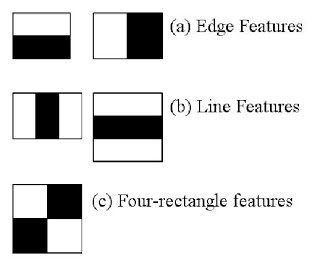
\includegraphics[scale=0.75]{haarfeature.jpg}}
\caption{Haar features used by OpenCV, a highly popular open-source computer vision library}
\label{haarfeature}
\end{figure}

Haar features work by taking the difference of the sum of the pixels inside two to four adjacent rectangles (depicted in Figure \ref{haarfeature}). The values can indicate characteristics about the image within the bounds of the rectangles, and these characteristics can be assessed or evaluated using machine learning algorithms (popularly AdaBoost \cite{FiveCuimei,NineHirzi}, but some use neural networks \cite{OneRadzi,EightRazzaq}).
	In Gupta et al. \cite{ThreeGupta}, researchers actually use Haar feature-based cascade classifiers on a Rpi as a precursor to face recognition, first detecting the face, then attempting to recognize it. The experiment was run on a Raspberry Pi 3B+ development kit with a processor that runs at 1.4Ghz, which slightly better performance compared to the Intel Pentium III used by Viola and Jones \cite{SixViola}, which was a generic desktop CPU at the time, which shows promise for the research done in this very paper. 
	Image size is also an important factor to consider when assessing performance. In Viola and Jones’s paper, they used 384 by 288 pixel images at 15 frames per second, and in Gupta et al. \cite{ThreeGupta}, the input image size and frames per second were notably not stated, however a webcam was used,  so it would be reasonable to infer that an average webcam in 2016 was what they used in that paper. 
	While this paper focuses on face detection, facial recognition may also be achievable, as shown by Radzi et al. \cite{OneRadzi} and Rouhsedaghat et al. \cite{FourRouhsedaghat}, where researchers assess the ability of a Rpi or other low-resource computing device to recognize faces. Typically this is achieved using some combination of neural networks and Principal Component Analysis, but in Rouhsedaghat et al. \cite{FourRouhsedaghat} they used PixelHop++ and successive subspace learning.

\begin{figure}[htbp]
\centerline{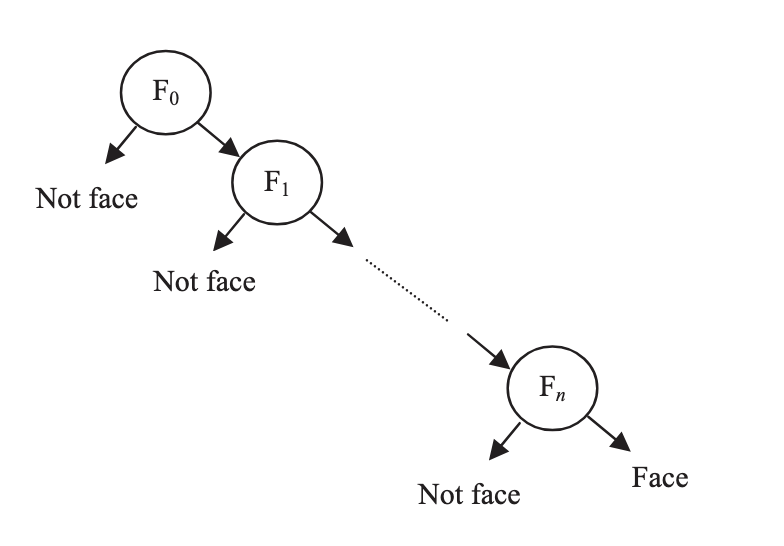
\includegraphics[scale=0.70]{haarcascade.png}}
\caption{Cascade model used in Haar feature-based cascade classification \cite{FiveCuimei}}
\label{cascademodel}
\end{figure}
\vspace{-10pt}
\section{Problem Statement}

Facial detection plays a key role in applications such as home security systems, smartphone cameras, and other IoT technologies. However, implementing reliable and efficient facial detection systems on devices with limited processing power like Raspberry Pi (Rpi) poses significant challenges. Other methods of face detection, such as neural networks, may be too computationally expensive for real-time processing required of IoT applications. In order to reach these speed requirements, a more efficient method must be used. Therefore, utilizing Haar feature-based cascade classifiers satisfies this requirement with a lightweight solution for facial detection.
In this project, we will investigate the use of Haar feature-based cascade classifiers for facial detection on a Raspberry Pi, focusing on finding a balance between facial detection accuracy and computational efficiency. The goal is to provide a practical and affordable facial detection system that can be implemented  in IoT-related solutions. Specifically, we aim to address the following questions:
\begin{itemize}
\item{\emph{How effective is the Raspberry Pi as a platform for facial detection using Haar classifiers, considering its hardware limitations?}}
\item{\emph{Can the facial detection system meet the real-time processing requirements necessary for IoT applications, such as home security?}}
\end{itemize}
By looking into these questions, we aim to assess the practicality of facial detection applications on Raspberry Pi using Haar feature-based cascade classifiers.

\begin{figure}[htbp]
\centerline{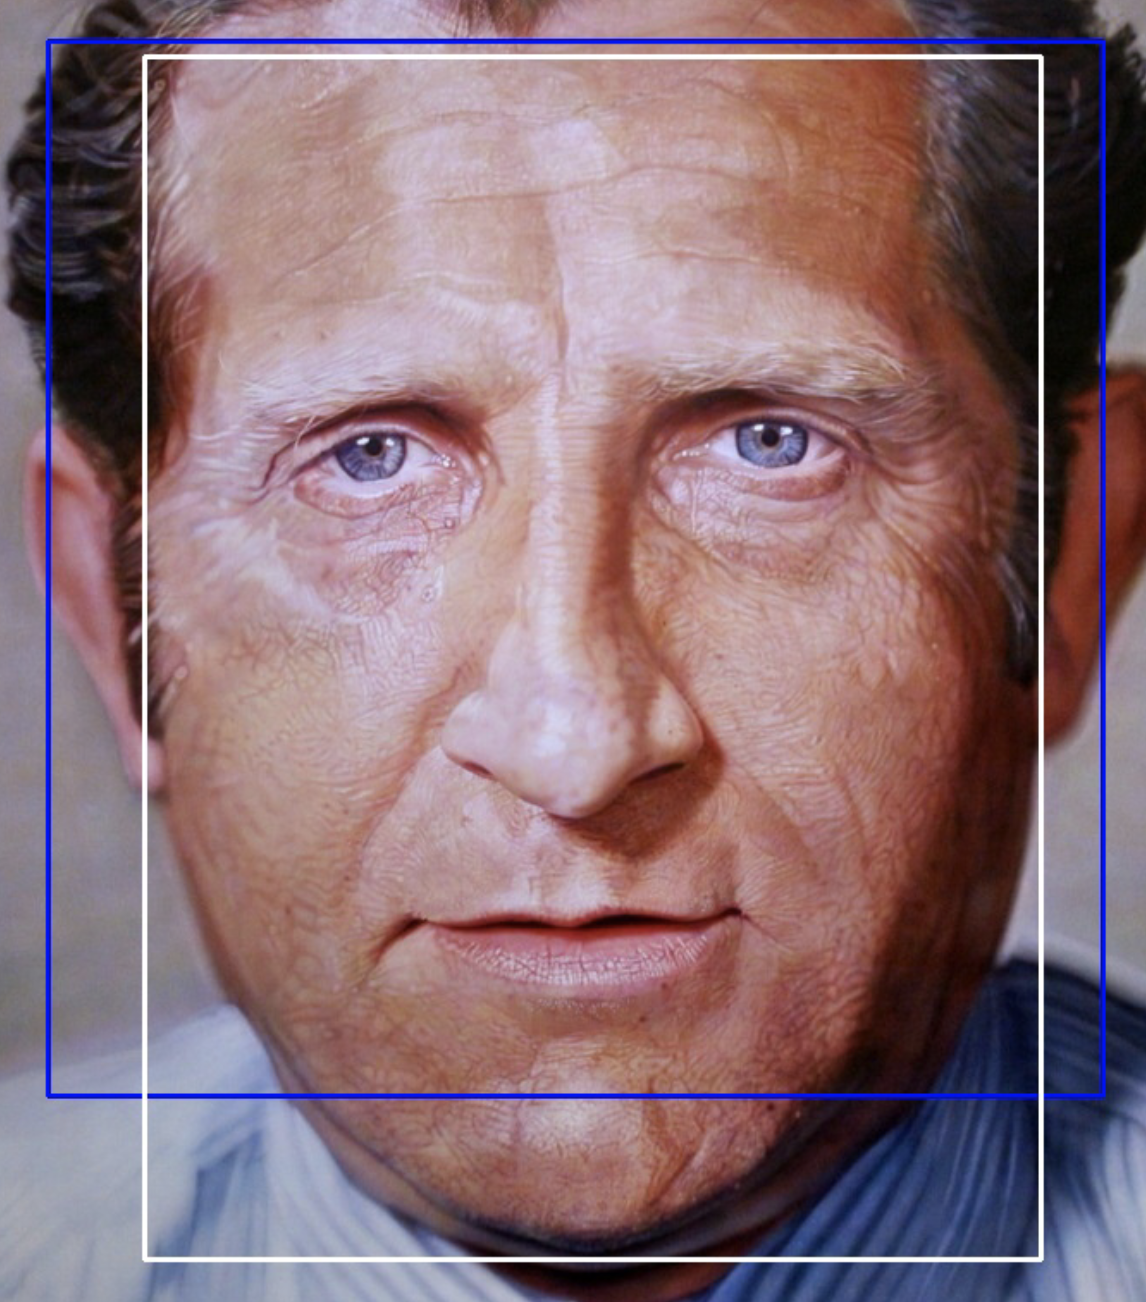
\includegraphics[scale=0.4]{IOU.png}}
\caption{Two bounding boxes, prediction by the model in blue, annotation in white. }
\label{example_iou}
\end{figure}
\vspace{-10pt}
\section{Method}
We will assess the performance of face detection using a Haar feature-based cascade classifier by measuring the model’s ability to detect faces, as well as the computational performance of a basic Python program that uses the model to detect faces in each frame of a live video feed. Model training is computationally expensive, and out-of-scope for the average non-expert looking to implement a face detection system for a home security system. However, while this paper is more focused on the hardware aspect of face detection, model performance is an important consideration when designing a face detection system. As such we decided to measure the performance of the particular model we used: OpenCV’s pre-trained \texttt{haarcascade\_frontalface\_default.xml} model. After assessing the model's performance, we measured CPU and memory utilization of a basic Python program, as well as measure the amount of time it takes to perform face detection on a single live video frame in the same program.

\subsection{Model Performance}
Intersection over Union (IoU) is a popular evaluation metric used in object detection \cite{IOURezatofighi}. It is computed by dividing the area of the intersection of two bounding boxes, by the area of the union. If the bounding boxes are entirely disjoint and do not overlap, the IoU is 0, and if the bounding boxes overlap perfectly, the IoU is 1. This can then be translated into more generalized performance measures like true positives (TP), false negatives (FN), and false positive (FP) by using a threshold value to determine the minimum IoU for a predicted object to be classified as TP. A FP is considered any prediction that does not exceed the IoU threshold, and a FN is any annotation that doesn't have a corresponding prediction. 

To give a complete picture of the model's performance, we measured the IoU for each predicted image and plotted a histogram, as well as plotted the precision and recall each threshold value between 0.00 and 1.00, in increments of 0.01. When considering images with multiple annotated and predicted faces, we had to consider how to assign predictions to annotations. Consider the scenario where there are two annotations and one prediction, with that prediction overlapping both annotations equally. We resolved this by computing an IoU value for all prediction-annotation, and selecting the pairs with the highest IoU, excluding pairs whose annotation or prediction had already been selected. The code we wrote to compute IoU for each prediction in an image can be found in our \href{https://github.com/etleyden/rpi-face-detection-research-project/blob/main/src/test_model.py}{repository on GitHub.}\footnote{\href{https://github.com/etleyden/rpi-face-detection-research-project}{Click this link to view the GitHub repo.}}

\begin{figure}[htbp]
\centerline{\includegraphics[scale=0.14]{face_detection.png}}
\caption{A VCU student testing out face\_detection.py}
\label{face_detection_example}
\end{figure}

\subsection{CPU and Memory Performance}
CPU and memory utilization are common metrics when considering the computational performance of a program. We devised \href{https://github.com/etleyden/cmsc436-research-paper/blob/main/src/face_detection.py}{a basic Python script (face\_detection.py)} that displays a live video feed of a webcam or other connected camera (such as the Rpi Camera Module 2), and runs each frame though the face detection model. When a face is detected, a blue bounding box is added to the image where the model detected a face. We measured the CPU and memory utilization of face\_detection.py using \href{https://github.com/etleyden/cmsc436-research-paper/blob/main/src/test_utilization.py}{a separate script (test\_utilization.py)} that spawns face\_detection.py as a subprocess, and reports the CPU and memory utilization using the \href{https://pypi.org/project/psutil/}{\texttt{psutil} package.} 

In this paper, CPU utilization is given as a sum of the percent utilization for each core. For example, if one core is being used 75\%, and another 80\%, then the total utilization is given as 155\%. Memory utilization is given in MB. While face\_detection.py is runnning, test\_utilization.py prints the CPU and memory utilization to the console once per second. When face\_detection.py is terminated, test\_utilization outputs the minimum, maximum, and average CPU and memory utilization to stdout. 

When listing the results for each computer used in this study, they will be listed by the names given in Figure \ref{hardware_specs}. The relevant hardware specifications for each computer are given in Figure \ref{hardware_specs} as well. 
\begin{figure}[htbp]
\begin{center}
\begin{tabular}{|r|>{\raggedright\arraybackslash}m{7.5em}|>{\raggedright\arraybackslash}m{6em}|} \hline
Computer Name & CPU & Memory Capacity \\ \hline
Raspberry Pi 3B+ & Broadcom BCM2837B0, Cortex-A53 (ARMv8) 64-bit SoC & 1GB LPDDR2 SDRAM \\ \hline
2019 Macbook Pro & Intel i7-9750H & 16GB DDR4 \\ \hline
2021 Macbook Pro & M1 Pro (Apple Silicon) & 16GB LPDDR5 \\ \hline
2021 Acer Swift & Intel i7-1165G7 & 16GB LPDDR4X \\ \hline
2022 Macbook Air & M2 (Apple Silicon) & 8GB LPDDR5 \\ \hline
\end{tabular}
\caption{Hardware specifications for each computer used in this study}
\captionsetup{justification=centering}
\label{hardware_specs}
\end{center}
\end{figure}
\vspace{-10pt}
\subsection{Frame-By-Frame Performance}
In addition to CPU and memory utilization, we also measured the elapsed time taken to detect faces within a frame. This code is written directly in face\_detection.py, and is run when the \texttt{-t} argument is passed to the program. When the argument is given, Python's built-in \texttt{time} module is used to measure the elapsed time taken to a) receive the image from the camera, and b) detect the faces. Any computation done after the face detection, between frames, is irrelevant to the face detection aspect itself and, as such, is not measured. The built-in timer \emph{does not} measure the elapsed time to  draw the returned bounding box on the image, print to stdout that a face was detected, and display the image on the screen. The results for each frame are then aggregated into minimum, maximum, and average milliseconds elapsed to perform face detection -- grouped by the number of faces detected in a frame. In other words, the program will report the minimum, maximum, and average milliseconds elapsed to detect faces for all frames with 0 faces, 1 face, 2 faces, etc. up to the maximum number of faces detected in a frame throughout the runtime of the program.

\begin{figure*}[t]
\centering
\begin{minipage}{0.90\textwidth}
\centering{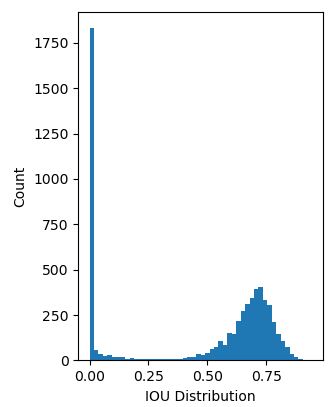
\includegraphics[scale=0.40]{model_result/val_iou_untrimmed.png}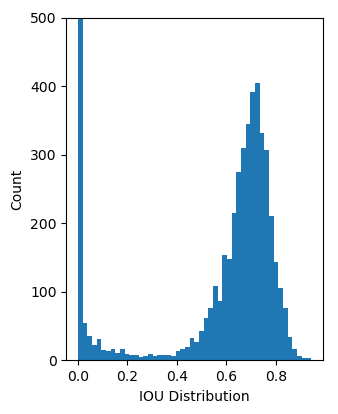
\includegraphics[scale=0.40]{model_result/val_iou_trimmed.png}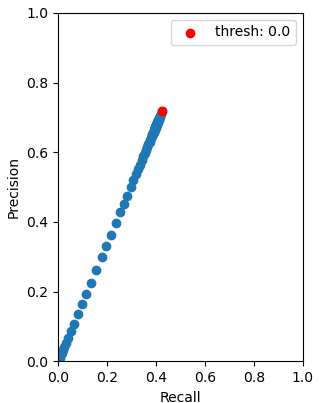
\includegraphics[scale=0.40]{model_result/val_precision.png}}
\caption{Results on the validation set.}
\captionsetup{justification=centering}
\label{validation_result}

\centering{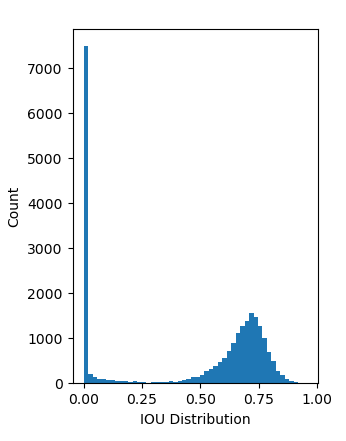
\includegraphics[scale=0.40]{model_result/train_iou_untrimmed.png}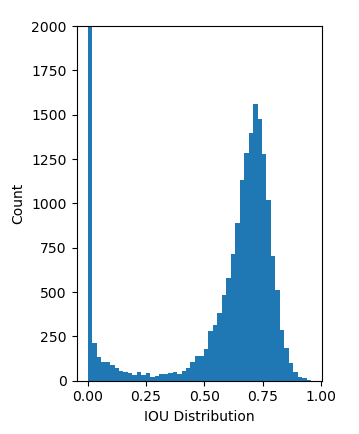
\includegraphics[scale=0.40]{model_result/train_iou_trimmed.png}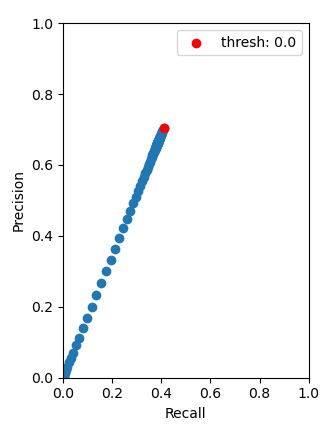
\includegraphics[scale=0.40]{model_result/train_precision.png}}
\caption{Results on the training set.}
\captionsetup{justification=centering}
\label{test_result}
\end{minipage}
\end{figure*}

\section{Results}

\subsection{Model Performance}

Shown in Figure \ref{validation_result} are the results of classification with \texttt{haarcascade\_frontalface\_default.xml} on the validation images, and in Figure \ref{test_result} are the results on the training images. On the left and center graphs, the IoUs of each predicted face are plotted on a histogram on the interval [0, 1] with a bucket size of 0.05. The left graph has an unaltered y-axis to give a complete picture of the predicted faces, and the center graph has an adjusted y-axis to more clearly show the distribution of valid detections. 

A "valid detection" is any detection that had a calculated IoU greater than 0. It is possible to adjust our definition on position of a false positive by choosing a value within the IoU interval as a threshold, and classifying anything greater than or equal to the threshold as a true positive, and anything below as a false positive. The rightmost graph is a plot of recall and precision for possible IoU thresholds on [0.01, 1.00] at an interval of 0.01. Highlighted in red is the precision and recall for the threshold with the highest F1 score (0.00). Note that a threshold of 0.00 inevitably includes false positives, which is discussed in more detail in the Discussion section. 

\begin{figure}[htbp]
\centering
\begin{tabular}{|r|c|c|} \hline
  & Validation & Training \\ \hline
Image Count & 3347 & 13386 \\ \hline
Pred. Faces & 6096 & 24155 \\ \hline
False Positives & 27.12\% & 28.47\% \\ \hline
Mean IoU (w/ FP) & 0.4582 & 0.4503 \\ \hline
Mean IoU (w/o FP) & 0.6287 & 0.6295 \\ \hline 
Std. Dev (w/o FP) & 0.2008 & 0.2012 \\ \hline
Recall (T:0.00)& 0.4206 & 0.4063 \\ \hline
Precision (T:0.00) & 0.7106 & 0.6989 \\ \hline
F1 (T:0.00) & 0.5285 & 0.5139 \\ \hline
Recall (T:0.01)& 0.4170 & 0.4038 \\ \hline
Precision (T:0.01) & 0.7046 & 0.6946 \\ \hline
F1 (T:0.01) & 0.5239 & 0.5107 \\ \hline
\end{tabular}
\caption{Statistics on model performance}
\captionsetup{justification=centering}
\label{tabulated_model_results}
\vspace{-2em}
\end{figure}

The histograms reveal a notable distribution pattern, with a significant portion of IoU values being concentrated at 0, indicating the presence of false positives. 27.12\% of the 6096 predictions on the validation set were false positives. Because the proportion of false positives to the rest of the dataset were so high, the distribution metrics we considered such as mean and standard deviation were skewed down, so in our distribution analysis, we filtered out all 0 IoU values from our calculations to focus on predictions that shared some overlap on the ground truth (the annotated data). Excluding false positive IoU's raise the mean IoU from 0.4582 to 0.6287, which more closely indicates the quality of bounding boxes on valid detections. 

Figure \ref{tabulated_model_results} presents a comprehensive summary of the experimental results evaluating model performance. The table includes key metrics such as the number of images processed, the total number of predicted faces, and the proportion of predictions classified as definite false positives (where IoU equals 0). Additionally, it provides the mean IoU values calculated both with and without false positives (denoted as "w/ FP" and "w/o FP," respectively) and the standard deviation of IoU values excluding false positives. Finally, recall, precision, and F1 scores are reported for two specific thresholds: 0.00, which yielded the highest F1 score, and 0.01, which more closely aligns with predictions matching the ground-truth annotations.

\subsection{CPU and Memory Performance}

In Figure \ref{cpu_mem_perf}, the results from our experiment of running a face detection program are listed. For each computer, the program \texttt{face\_detection.py} was run for approximately 5 minutes, and intermittently presented anywhere from 0 to 5 faces. The maximum and average CPU and memory utilization are presented, and the minimum is excluded from this paper since the value is more representative of the state of the machine at the beginning of the runtime of the program, and does not provide meaningful insight into system performance during runtime. The results from the Raspberry Pi are listed first and emphasized, since that platform is the focus of the paper. 
\begin{figure}[htbp]
\begin{center}
    \begin{tabular}{| >{\raggedright\arraybackslash}m{8em} |c|c|c|c|} \hline
         & \multicolumn{2}{|c|}{CPU (\%) } & \multicolumn{2}{|c|}{Memory (MB)} \\ \hline
         & Max & Mean & Max & Mean \\ \hhline{|=|=|=|=|=|}
    \textbf{\emph{Raspberry Pi 3B+}} & \textbf{\emph{367.7}} & \textbf{\emph{305.3}} & \textbf{\emph{147.1}} & \textbf{\emph{141.5}} \\ \hline
    2019 Macbook Pro & 767.0 & 609.5 & 136.5 & 126.5 \\ \hline
    2021 Macbook Pro & 408.1 & 356.6 & 434.9 & 354.7 \\ \hline
    2021 Acer Swift & 539.1 & 398.8 & 162.8 & 161.0 \\ \hline
    2022 Macbook Air & 388.0 & 332.9 & 335.6 & 331.6 \\ \hline
    \end{tabular}
        \caption{CPU and memory utilization for various computers}
        \captionsetup{justification=centering}
        \label{cpu_mem_perf}
        \end{center}
        \vspace{-14pt}
\end{figure}

\subsection{Frame-By-Frame Performance}

Finally, in our analysis of frame-by-frame performance, we have plotted the maximum, average, and minimum values in Figures \ref{max_fbf_perf}, \ref{avg_fbf_perf}, and \ref{min_fbf_perf} respectively. To save space on the plots, we've abbreviated the names of each device in the legend. "Macbook Pro" was abbreviated to "MBP", "Macbook Air" to "MBA", "Raspberry Pi 3B+" to "Rpi", and "Acer Swift" to "AS". These are the same computers used in the CPU and memory utilization experiments. Note that y-axis of the minimum plot, Figure \ref{min_fbf_perf} has been adjusted to more clearly show the differences between devices, and is different than the y-axis in Figures \ref{max_fbf_perf} and \ref{avg_fbf_perf}. Since the Raspberry Pi is the primary platform of our study, results from the device are in bright green, intentionally chosen for its visual prominence.


% max plot
\begin{figure}[htbp]
\begin{center}
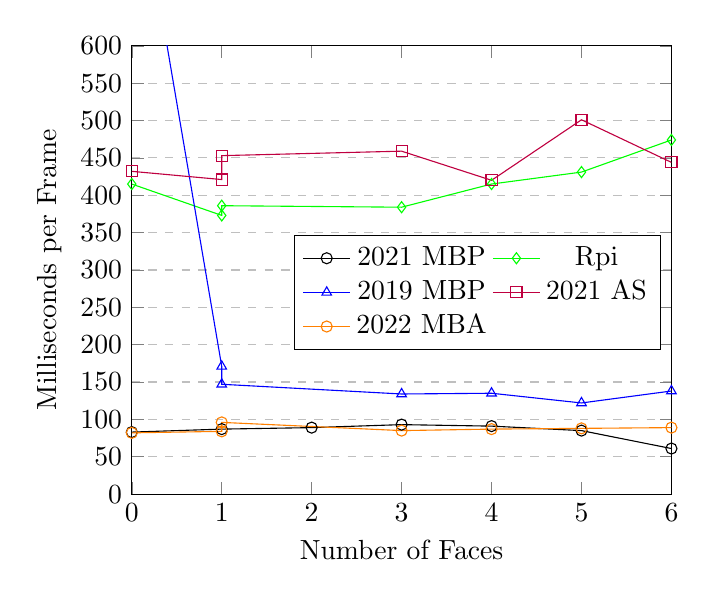
\begin{tikzpicture}
    \begin{axis}[
        xlabel={Number of Faces},
        ylabel={Milliseconds per Frame},
        xmin=0, xmax=6,
        ymin=0, ymax=600,
        xtick={0,1,2,3,4,5,6},
        ytick={0,50,100,150,200,250,300,350,400,450,500,550,600},
        legend style={
            at={(0.3,0.45)},
            anchor=west
        },
        legend columns=2,
        ymajorgrids=true,
        grid style=dashed,
    ]

    \addplot[
        color=black,
        mark=o,
        ] coordinates {
            (0,83) (1,87) (2,89) (3,93) (4,91) (5,85) (6,61)
        };
    \addlegendentry{2021 MBP}
    \addplot[
        color=green,
        mark=diamond,
        ] coordinates {
            (0,415) (1,373) (1,386) (3,384) (4,415) (5,431) (6,474)
        };
    \addlegendentry{Rpi}
    \addplot[
        color=blue,
        mark=triangle,
        ] coordinates {
            (0,877) (1,171) (1,147) (3,134) (4,135) (5,122) (6,138)
        };
    \addlegendentry{2019 MBP}
    \addplot[
        color=purple,
        mark=square,
        ] coordinates {
            (0,432) (1,421) (1,453) (3,459) (4,420) (5,501) (6,444)
        };
    \addlegendentry{2021 AS}
    \addplot[
        color=orange,
        mark=o,
        ] coordinates {
            (0,82) (1,84) (1,96) (3,85) (4,87) (5,88) (6,89)
        };
    \addlegendentry{2022 MBA}
    
    \end{axis}
\end{tikzpicture}
        \caption{Maximum frame by frame performance}
        \captionsetup{justification=centering}
        \label{max_fbf_perf}
% avg plot
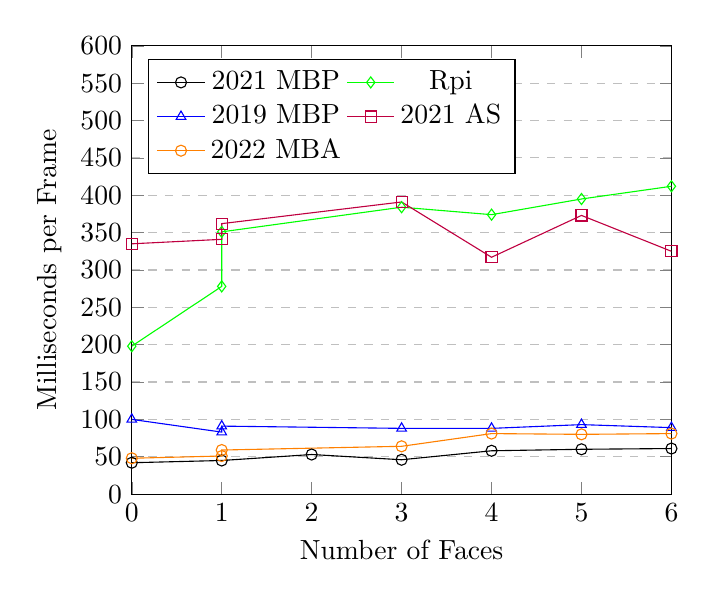
\begin{tikzpicture}
    \begin{axis}[
        xlabel={Number of Faces},
        ylabel={Milliseconds per Frame},
        xmin=0, xmax=6,
        ymin=0, ymax=600,
        xtick={0,1,2,3,4,5,6},
        ytick={0,50,100,150,200,250,300,350,400,450,500,550,600},
        legend pos=north west,
        legend columns=2,
        ymajorgrids=true,
        grid style=dashed,
    ]

    \addplot[
        color=black,
        mark=o,
        ] coordinates {
            (0,42) (1,45) (2,53) (3,46) (4,58) (5,60) (6,61)
        };
    \addlegendentry{2021 MBP}
    \addplot[
        color=green,
        mark=diamond,
        ] coordinates {
            (0,198) (1,278) (1,351) (3,384) (4,374) (5,395) (6,412)
        };
    \addlegendentry{Rpi}
    \addplot[
        color=blue,
        mark=triangle,
        ] coordinates {
            (0,100) (1,83) (1,91) (3,88) (4,88) (5,93) (6,89)
        };
    \addlegendentry{2019 MBP}
    \addplot[
        color=purple,
        mark=square,
        ] coordinates {
            (0,335) (1,341) (1,362) (3,391) (4,317) (5,373) (6,325)
        };
    \addlegendentry{2021 AS}
    \addplot[
        color=orange,
        mark=o,
        ] coordinates {
            (0,48) (1,51) (1,59) (3,64) (4,81) (5,80) (6,81)
        };
    \addlegendentry{2022 MBA}
    
    \end{axis}
\end{tikzpicture}
        \caption{Average frame by frame performance}
        \captionsetup{justification=centering}
        \label{avg_fbf_perf}
% min plot
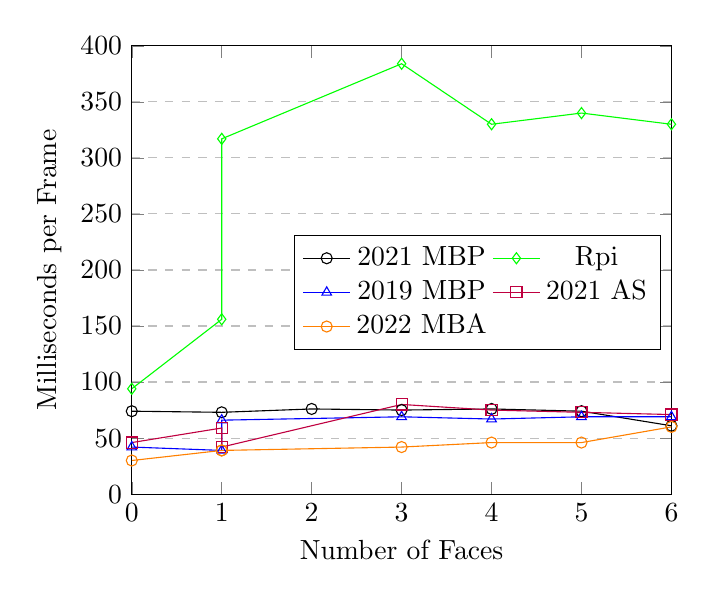
\begin{tikzpicture}
    \begin{axis}[
        xlabel={Number of Faces},
        ylabel={Milliseconds per Frame},
        xmin=0, xmax=6,
        ymin=0, ymax=400,
        xtick={0,1,2,3,4,5,6},
        ytick={0,50,100,150,200,250,300,350,400},
        legend style={
            at={(0.3,0.45)},
            anchor=west
        },
        legend columns=2,
        ymajorgrids=true,
        grid style=dashed,
    ]

    \addplot[
        color=black,
        mark=o,
        ] coordinates {
            (0,74) (1,73) (2,76) (3,75) (4,76) (5,74) (6,61)
        };
    \addlegendentry{2021 MBP}
    \addplot[
        color=green,
        mark=diamond,
        ] coordinates {
            (0,94) (1,156) (1,317) (3,384) (4,330) (5,340) (6,330)
        };
    \addlegendentry{Rpi}
    \addplot[
        color=blue,
        mark=triangle,
        ] coordinates {
            (0,42) (1,39) (1,66) (3,69) (4,67) (5,69) (6,69)
        };
    \addlegendentry{2019 MBP}
    \addplot[
        color=purple,
        mark=square,
        ] coordinates {
            (0,46) (1,59) (1,42) (3,80) (4,75) (5,73) (6,71)
        };
    \addlegendentry{2021 AS}
    \addplot[
        color=orange,
        mark=o,
        ] coordinates {
            (0,30) (1,39) (1,39) (3,42) (4,46) (5,46) (6,60)
        };
    \addlegendentry{2022 MBA}
    
    \end{axis}
\end{tikzpicture}

        \caption{Minimum frame by frame performance}
        \captionsetup{justification=centering}
        \label{min_fbf_perf}
        \end{center}
\end{figure}

\section{Discussion}

\subsection{Model Performance}

In our evaluation of model performance, we predicted faces on two annotated datasets by evaluating a larger dataset's validation and training set separately. Note that the training set contains more than four times the number of images in the validation set, which has the potential to indicate patterns on the model's predictions as the volume of data increases. First we evaluated the model performance independent of input volume by analyzing the results on the training set -- since larger datasets are generally more representative of real-world distributions. Then, in the section "Performance Trends with Increased Data Volume" we compared the two datasets, and analyzed how the performance results changed as the input volume increased. 

\subsubsection{General Performance Trends}
The false positive rate on the training set was high at 28.47\%. This is over a fourth of the predicted faces within each image set. High false positive rates are consistent across haar cascade classifiers \cite{FiveCuimei,SixViola,EightRazzaq}, and this could potentially be improved if we chose a different model \cite{NN_accuracy}. This study is focused on the hardware aspects of face detection, but an analysis of multiple models could provide valuable insights, and could be an avenue for further research. 

A "valid detection" is not strictly limited to any prediction with an IoU greater than 0.00. The threshold can be adjusted, with higher IoU thresholds imposing stricter requirements for the overlap between predicted and ground truth bounding boxes. We analyze the accuracy as the threshold increases from 0.00 to 1.00 by plotting the precision and recall for every threshold in that range on increments of 0.01, as well as plotting the IoU for all predictions on a histogram. Figure \ref{test_result} depicts those plots for the training set, but the validation set is notably similar. 

The mean IoU excluding 0.00 on the training set is 0.6295, which is noticeably lower than the peak of the curve on the histogram. This can be attributed to the slight skew of predictions. As previously stated, the false positive rate of the model was high (more than a fourth of predictions did not overlap with any annotations), but it is even higher than that if you increase the threshold to the local minimum (approximately 0.25). On the training set, the false positive rate increases almost 5\%, from 28.47\% to 34.77\%.

The predictive performance of face detection models can be difficult to quantify in comparison to simple classification models. Popular metrics include Intersection-over-Union, but also include more familiar metrics like precision, recall, and F1 score. In Figure \ref{test_result}, we've plotted the precision and recall for thresholds in the range [0.00, 1.00] on an interval of 0.01. As the threshold decreases, precision and recall share a linear non-decreasing relationship, peaking at a maximum precision of 0.6989 and recall of 0.4038 on the training set. The F1 score of the model, with a threshold of 0.00 is 0.5139. The F1 score excluding false positives is intuitively lower, albiet only slightly, with an F1 score of 0.5107 at a threshold of 0.01. The biggest change in F1 score are in fact when the threshold is increases through the range where the majority of the IoU values are concentrated. This trend is evident on the plot of precision and recall where the increased spacing between points along the line correspond to the primary curve of the IoU distribution.

\subsubsection{Performance Trends with Increased Data Volume}
Nearly every statistic that we measured during our predictive performance analysis showed that performance decreased as the volume of input to the model increased, however only slightly. From the validation to the training set, the input volume increased by 400\% (quadrupled). The slight decrease in performance could possibly indicate a small discrepancy between our analysis and real-world results, especially as the variability and edge cases found in the real world are encountered using the model we analyzed. 

The results on the predictive performance of \texttt{haarcascade\_frontalface\_default.xml} show that the model has a high tendency to predict false positives in general. For both the validation and training images, the proportion of IoU values equal to 0 for predicted faces were 27.12\% and 28.47\% respectively. The proportion of false positives increased by almost 1\%, as the number of predictions quadrupled, which could indicate that as the number of predicted faces increase, so does the proportion of false positives by a small (perhaps negligible) amount.

With the exception of the mean excluding false positives and standard deviation, every metric decreased slightly, implying worse performance on a wider range of data. The increase in standard deviation implies this also, since a higher standard deviation means a higher variation in predictive performance. 

\subsection{CPU and Memory Performance}

At first glance, the measured CPU and memory performance of \texttt{face\_detection.py} across various hardware platforms seem unintuitive. The program had the lowest CPU utilization on the Raspberry Pi, with an average CPU utilization of 305.3\%. The worst CPU utilization was on the 2019 Macbook Pro, where the mean CPU utilization was 609.5\% (more than six cores being used!). However this device had the lowest mean memory usage at 126.5MB. The worst memory usage was the 2021 Macbook Pro at 354.7MB.

We hypothesize that the explanation of these results lies in the implementation of OpenCV and how it may optimize performance depending on the available hardware. Additionally, various operating systems will make different resource allocation choices depending on the creators of those operating systems. For example, the creators of Raspberry Pi OS likely optimize resource allocation for low-resource environments when MacOS developers instead optimize resources to use the full resources available to them. To illustrate this point, consider that 141.5MB is one tenth of the available RAM on the Raspberry Pi in our experiment, but 354.7MB is a mere 2\%.

\subsection{Frame-By-Frame Performance}

Finally, we analyzed the frame-by-frame performance of each hardware platform by measuring the number of milliseconds it takes to process a frame and aggregating the results given the number of faces predicted within the frame. The first observation we had on the frame-by-frame results are that performance is largely consistent across the number of faces in frame among the Macbooks. The only exception to this is the maximum compute time for the 2019 Macbook Pro on 0 faces, which was unusally high. The unexpectedly high maximum processing time for a live video frame in the face detection program could be attributed to routine system-level factors. These include other system processes temporarily taking priority over the execution of \texttt{face\_detection.py}, leading to resource contention. Additionally, anomalies occurring during the program's initialization, such as delays in allocating memory or initializing dependencies, may have contributed to the observed outliers in processing time. These factors highlight the influence of non-deterministic operating system behaviors on real-time performance, even when ample resources are available. 

The second observation is that the compute time on the Raspberry Pi is significantly slower than almost any other platform in our study, which is consistent with expectations. Average compute time for a single frame was between a third and a half of a second, which is an important factor to consider when designing a home security system involving face detection. The only platform that occasionally exceeded the Raspberry Pi in compute time was the 2021 Acer Swift, which upon further investigation was running 100+ Google Chrome tabs. This finding highlights the impact of system resource contention and background processes on compute performance, even for hardware designed with more substantial capabilities.

\section{Conclusion}

Overall the results of this study demonstrate that it is generally feasible to use a Raspberry Pi as tool for face detection in a home security environment. At the time of writing, a Raspberry Pi 3B+ is \href{https://www.adafruit.com/product/3775?src=raspberrypi}{available from Adafruit} for \$35, and the Raspberry Pi Camera Module V2 is \href{https://a.co/d/0I5FcZJ}{available from Amazon} for \$17.41, which means that the cost of a do-it-yourself (DIY) implementation is just over \$50. While indoor/outdoor security cameras range from just under \$20 to more than \$100 per camera, most do not offer the same degree of freedom as a DIY solution, and many cameras are connected to the manufacturers' infrastructure on the basis of providing live video feeds accessible over the internet, and recordings that are saved to the cloud. In a DIY solution, an amateur home security system could provide services on par with current solutions on the market for the average consumer. 

Concerning predictive performance, the model's ability to reliably identify faces is questionable. In the context of home security, a DIY home security system may be required to recognize faces at a distance, at an angle, or in another scenario where the live video feed may be distorted. If the homeowner expects a highly accurate face detection system, they should look elsewhere. With a high false positive rate, it would be inadvisable to expect that every detected face is a legitimate detection.

There exists a plethora of research topics that could potentially expand the results of this study. Namely, future research could focus on the accuracy or performance of different face detection models, other home security uses of a Raspberry Pi, or feasibility of expanding the rudimentary face detection program we have written for this paper. The findings of this study highlight the trade-offs between computational efficiency and predictive accuracy, emphasizing the need for optimized hardware-software integration to enhance the real-world applicability of face detection algorithms on resource-constrained devices like the Raspberry Pi.
\section{References}
\renewcommand{\refname}{}  % Suppress the default unnumbered title for article class
% \renewcommand{\bibname}{}  % Uncomment this for report or book class
\bibliographystyle{IEEEtran}
\bibliography{ref}
\vspace{12pt}

\end{document}
